\chapter{Manuel de la maquette}

\section{Protocole de mise en service}
\label{sec:Protocole}
La mise en service de la maquette s’effectue selon la procédure suivante :
\begin{enumerate}
    \item Allumer l’alimentation 48 V en réglant la limitation de courant à 3,5 A. Pour ajuster cette limite, presser le bouton de réglage correspondant sur l’alimentation.

    \item Compiler et charger la dernière version du code depuis Code Composer Studio vers le DSP.

    \item Configurer l’oscilloscope sur la résistance de charge des cartes de puissance (calibres : 50 ms/div et 10 V/div pour les deux sondes). Placer le trigger du canal mesurant le côté électrique de la résistance, vers les cartes de puissance, à 20 V. Régler l’oscilloscope en mode « Single » afin d’observer la charge des condensateurs lors de l’enclenchement de l’interrupteur S1.

    \item Une fois la tension de 48 V établie et le transistor commuté, presser le bouton physique S2 ou cliquer sur le bouton \textit{Start} dans l’onglet « Mise en marche » de l’interface logicielle pour lancer la sustentation.
\end{enumerate}

\section{Calibration des capteurs de position}
\label{sec:CalibrationCaptPos}
Les capteurs de position disposent d’une calibration appelée « Teach-in ». De plus amples détails sur cette méthode sont présentés dans l’annexe \cite{CaptPosition}.

Les étapes pour réaliser une calibration selon la méthode « Teach-in » sont les suivantes :

\begin{enumerate}
    \item Presser la touche. La LED rouge s’allume lorsque l’apprentissage du détecteur est encore possible.

    \item Presser la touche pendant 5 secondes jusqu’à ce que la LED rouge commence à clignoter.

    \item Relâcher la touche.

    \item Placer l’objet de mesure à la limite de la plage de mesure pour laquelle le détecteur doit afficher une valeur de 0 V, respectivement de 4 mA.

    \item Presser brièvement la touche. La LED rouge s’allume pendant 3 secondes comme confirmation. Ensuite, elle se remet à clignoter de façon régulière.

    \item Placer l’objet de mesure à la limite de la plage de mesure pour laquelle le détecteur doit afficher une valeur de 10 V, respectivement de 20 mA. Presser brièvement la touche. La LED rouge s’allume pendant 3 secondes comme confirmation. Ensuite, elle s’éteint pour clignoter encore une fois brièvement. Le détecteur est alors de nouveau opérationnel.
\end{enumerate}

La seconde mesure, correspondant à la distance minimale, doit toutefois être réalisée suffisamment rapidement pour permettre au capteur d’enregistrer cette valeur.

Afin de faciliter la mesure, un programme réalisant uniquement une régulation de courant constant est utilisé. Ce programme est disponible dans Test\_pour\_carte\_principale\_4\_inducteurs\textbackslash Fichier\_de\_test\textbackslash Test\_regulation\_courant.c. L’emploi de ce code permet d’appliquer les électroaimants aux rails afin d’obtenir un entrefer de 0 mm. Pour enclencher les électroaimants, il suffit d’appuyer sur le bouton. À ce moment-là, une LED s’allume et indique le début de la régulation. Une fois cette étape réalisée, il suffit de soulever les inducteurs à la main en les tenant par les pieds jusqu’à leur contact avec le rail. Les quatre inducteurs doivent impérativement être collés afin d’éviter la création d’un angle susceptible de fausser la mesure. Lorsque les électroaimants sont collés, les étapes précédentes peuvent être suivies pour réaliser le teach-in. Lorsque la plage minimale a été enregistrée, il suffit d’appuyer une nouvelle fois sur le bouton pour faire abaisser les électroaimants. La plage maximale du capteur peut alors être enregistrée.

Une fois cette procédure terminée, le capteur est calibré.

\subsection{Configuration de CCS}

Une fois l'installation terminée, il est nécessaire de configurer CCS pour qu'il détecte la bibliothèque. La procédure d'intégration est la suivante :

\begin{enumerate}
    \item Lancer Code Composer Studio.

    \item Accéder au menu \textit{Window > Preferences}.

    \item Dans la colonne de gauche, naviguer vers \textit{Code Composer Studio > Products}.

    \item Vérifier la liste "Product discovery path". Si le dossier \verb|C:\ti| n'y figure pas, cliquer sur \textit{Add...} et le sélectionner.
    \item Cliquer sur le bouton \textit{Refresh}.

    \item La bibliothèque C2000Ware doit apparaître dans la liste « Discovered products ». Cliquer alors sur \textit{Install}.

    \item Si l'explorateur de fichiers s'ouvre, sélectionner l'emplacement exact du dossier (généralement \verb|C:\ti\c2000\C2000Ware_5_02_00_00|).

    \item Vérifier que le dossier est correctement coché et cliquer sur \textit{Apply and close}. La figure \ref{fig:Res_conf_C2000} illustre le résultat attendu.

          \begin{figure}[H]
              \centering
              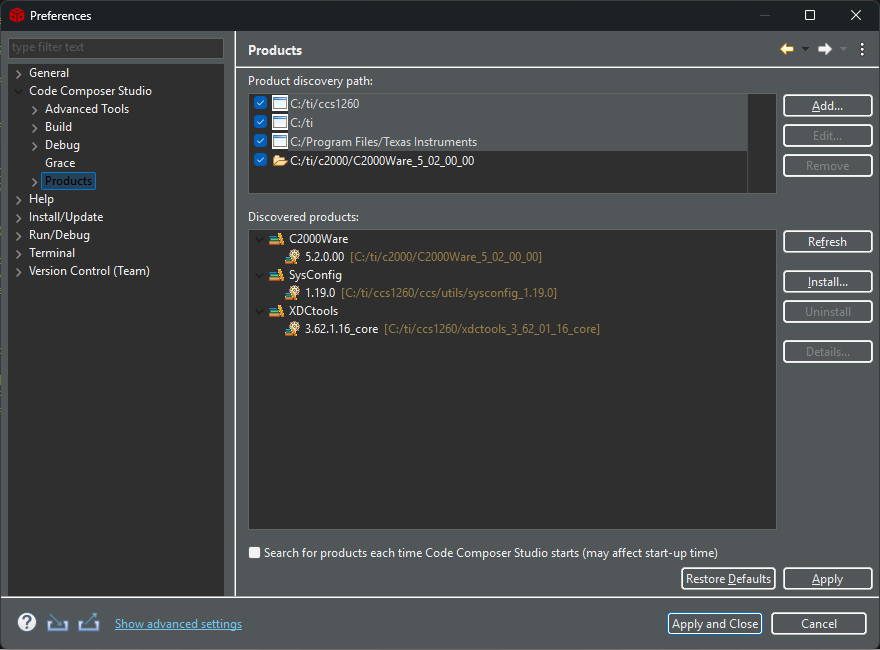
\includegraphics[width=0.75\linewidth]{Image/Chap.2/Resultat_conf_C2000.png}
              \caption{Résultat de la configuration du C2000}
              \label{fig:Res_conf_C2000}
          \end{figure}

    \item Une fois la configuration terminée, cliquer sur le bouton \textit{Build} pour appliquer les changements.
\end{enumerate}

Enfin, il est impératif de vérifier que le niveau d'optimisation de CCS est correctement établi en suivant ces étapes :

\begin{enumerate}
    \item Effectuer un clic droit sur le projet.

    \item Sélectionner \textit{Properties}.

    \item Dérouler l'onglet \textit{Build > C2000 Compiler > Optimization}.

    \item Appliquer les paramètres tels qu'illustrés dans la fenêtre suivante :

          \begin{figure}[H]
              \centering
              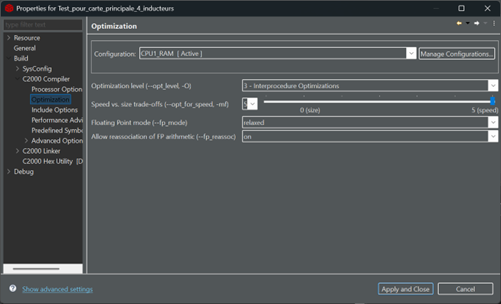
\includegraphics[width=0.75\linewidth]{Image/Chap.2/CCS_Opti_Windows.png}
              \caption{Configuration des paramètres d'optimisation}
              \label{fig:Res_conf_Opti}
          \end{figure}
\end{enumerate}

Lorsque le programme final est prêt, il faudra à ce moment-là flasher le code dans la mémoire flash afin que le code reste en "stand alone".

Il est désormais possible d'utiliser CCS pour la programmation du DSP.

\section{Affichage de l'interface WEB}
Afin de se connecter à l'interface, il est néscessaire de se connecter au WIFI créer par l'ESP-32. Pour cela, les informations suivantes sont néscessaire pour s'y connecter :

\begin{itemize}
    \item Nom du wifi : ESP32-S2-WIFI
    \item Mot de passe : TFE-TB2025-HEIG
    \item Lien du site web : 192.168.4.1
\end{itemize}

\clearpage